\section{Observational Properties} \label{sec:obs}
% ============================================================================
Throughout this section, each statistic is computed on the subset of the
$1057$ bins for which the relevant quantity is constrained: $792$ bins
($75\%$) have a physically valid Band fit (the reference for $\alpha$, \Ep,
and flux); $301$ bins have a decisive blackbody ($\daic\ge10$;
Section~\ref{sec:fit}), of which $233$ also have a valid Band flux; $349$ bins
have a valid 2SBPL with ordered breaks; $950$ bins have at least two
physically valid models (the model-comparison set); and per-burst statistics
use the $100$ bursts with at least one valid Band bin, with per-burst
correlations requiring $\ge$$5$ bins ($68$ bursts) or $\ge$$4$
$\Ep$--$\kT$ pairs ($19$ bursts).

\subsection{Parameter Distributions} \label{sec:dist}
We now examine the distributions of the spectral parameters
(Figure~\ref{fig:dist}, Table~\ref{tab:dist}). The low-energy index has a
median $\alpha=-0.71\pm0.49$, the peak energy $\log_{10}(\Ep/{\rm keV})=
2.28\pm0.40$ (median $\Ep\simeq192$~keV), and the high-energy index a median
$\beta=-2.6$, in agreement with previous catalogs
\citep[e.g.,][]{Kaneko2006,Gruber2014}. The blackbody temperature, where
decisively required, has a median $\kT\simeq28$~keV and spans
$\kT\approx3$--$70$~keV (5th--95th percentiles), bracketing the
$\sim$$40$~keV temperatures of \citet{Guiriec2015}. K-S tests between tiers
(Table~\ref{tab:ks}) show that the Gold-tier distributions differ modestly from
the lower tiers ($p\approx0.004$ for $\alpha$, $0.03$ for $\log\Ep$), as
expected since the brightest bursts populate the Gold tier; the difference does
not affect the conclusions below.

\begin{figure*}[t]
\centering
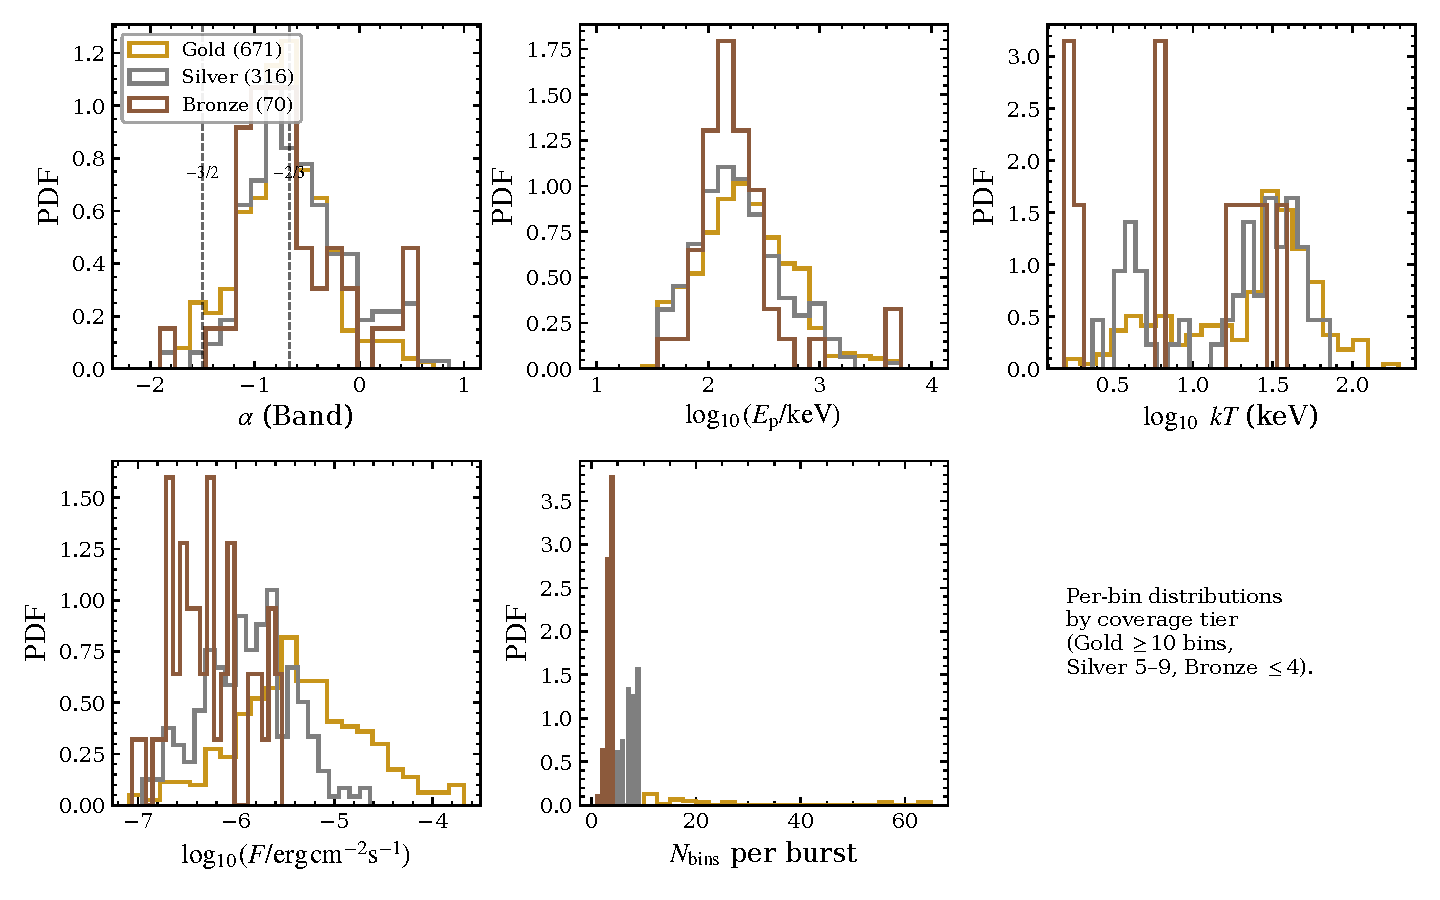
\includegraphics[width=0.95\textwidth]{two_break_figures/fig_dist.pdf}
\caption{Distributions of the Band low-energy index $\alpha$, peak energy \Ep,
blackbody temperature \kT, energy flux $F$, and the number of bins per burst,
split by coverage tier (Gold/Silver/Bronze). The legend gives the total number
of time bins per tier ($1057$ in all); each panel shows the subset in which the
plotted parameter is constrained. Dashed lines in the $\alpha$ panel mark the
slow- and fast-cooled synchrotron limits ($-2/3$, $-3/2$).}
\label{fig:dist}
\end{figure*}

\subsection{Spectral Evolution} \label{sec:evol}
We classify the \Ep\ evolution into hard-to-soft (HTS) and intensity-tracking
(IT) patterns following the physical discriminant of \citet{Lu2012} and
\citet{Basak2014}: the two classes differ in the \emph{rising} phase of the
pulse, where an IT pulse hardens with the flux while an HTS pulse is already at
its hardest and softening (in the decay phase both soften together, so a
whole-pulse $\Ep$--flux correlation cannot separate them). We therefore
classify on the pre-peak behavior---the sign of the $\Ep$ trend through the
flux peak, falling back to the position of the \Ep\ maximum when the rise is
covered by fewer than three bins. Of the $76$ bursts with $\ge$$4$ classifiable
bins, $63\%$ ($48/76$) are HTS, $25\%$ ($19/76$) are IT, and $12\%$ ($9/76$)
are ambiguous (Figure~\ref{fig:evol}), an HTS-dominated mix consistent with the
small single-pulse samples of \citet{Lu2012} and \citet{Basak2014}. The general
trend is that pulses soften over time, with $\alpha$ decreasing through the
pulse.

\begin{figure*}[t]
\centering
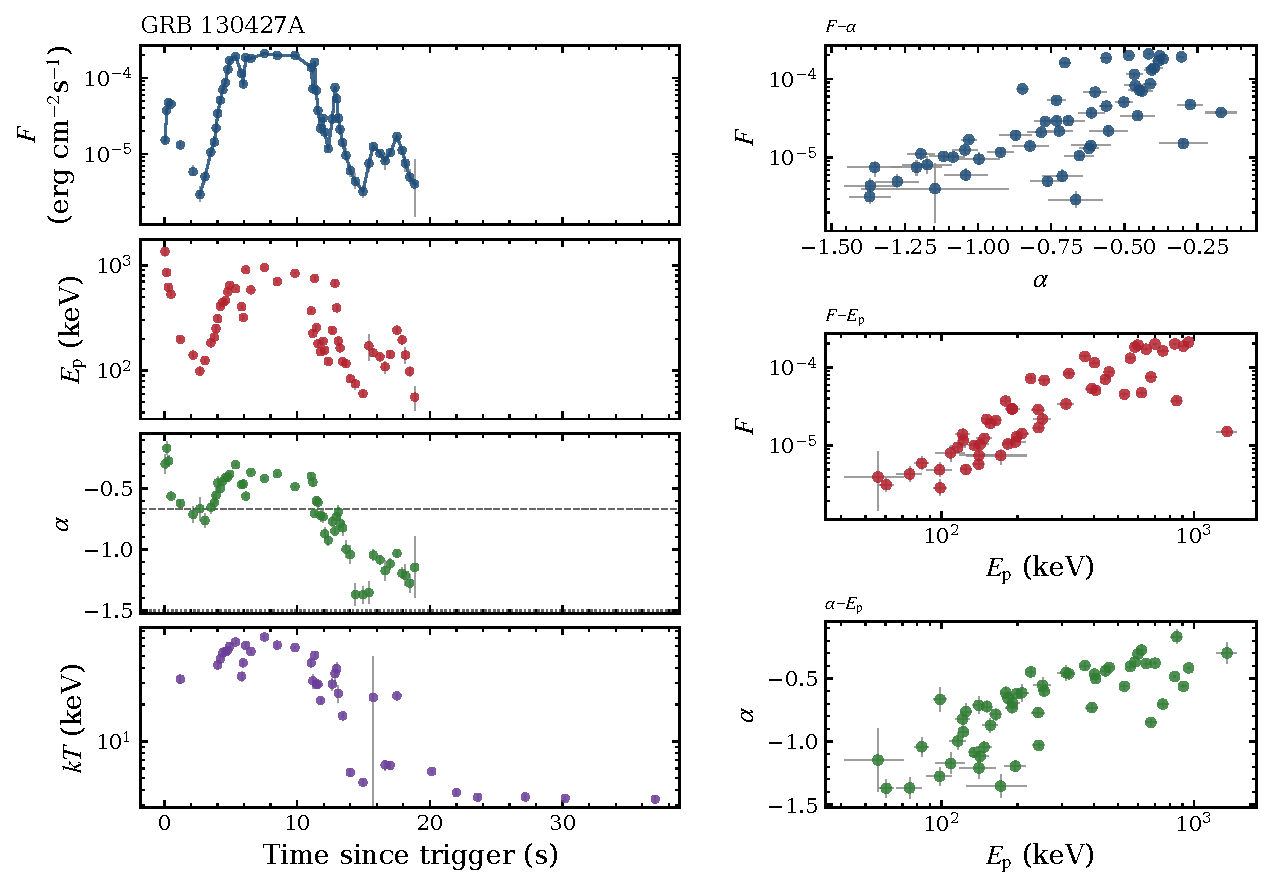
\includegraphics[width=\textwidth]{two_break_figures/fig_evol.pdf}
\caption{Time-resolved spectral evolution of GRB~130427A ($65$ bins in all).
Left, top to bottom: the energy-flux light curve $F(t)$, $\Ep(t)$, $\alpha(t)$
(dashed/dotted lines at $-2/3$, $-3/2$), and $\kT(t)$. Each panel shows the
bins in which the plotted quantity is constrained ($54$ Band-valid bins for
$F$, \Ep, $\alpha$; decisive-blackbody bins for $\kT$, which extend into the
late tail). Right: the $F$--$\alpha$, $F$--$\Ep$, and $\alpha$--$\Ep$ relations
for the same burst.}
\label{fig:evol}
\end{figure*}

\subsection{Parameter Correlations} \label{sec:corr}
Turning to the parameter correlations, we fit each pair with the functional forms
adopted by \citet{Li2021} and report both the per-burst incidence and the pooled,
sample-wide trend (Table~\ref{tab:curv}).

\subsubsection{The $F$--$\alpha$ Relation}
We fit $F=F_0\,e^{k\alpha}$ and find a positive correlation in $84\%$ ($57/68$)
of bursts, with pooled $k=0.27$: brighter spectra tend to have harder low-energy
indices, though the trend is weak (pooled $\rho=0.17$).

\subsubsection{The $F$--$\Ep$ Relation}
We fit a power law $F\propto\Ep^{\,k_1}$ and find $k_1=0.66$, positive in $94\%$
($64/68$) of bursts (pooled $\rho=0.43$). This correlation, however, is partly
\emph{induced}: the energy flux is $\int E\,N(E)\,dE$, which rises when \Ep\
shifts to higher energies even at a fixed photon rate, so part of any
$F$--\Ep\ correlation is built into the quantities themselves. In photon flux
(which carries no such energy weighting) the rank correlation collapses to
$\rho=0.15$, consistent with the absence of an intrinsic $\Ep$--luminosity
relation \citep{Mei2025}.

\subsubsection{The $\alpha$--$\Ep$ Relation}
We fit $\alpha=k_2\log_{10}\Ep+c$ and find only a weak positive trend,
$k_2=0.02$ (pooled $\rho=0.10$); a positive per-burst correlation appears in
$66\%$ ($45/68$) of bursts but is individually significant in only a handful.

\subsection{Curvature and the Two Pictures} \label{sec:curv}
We now turn to the curvature beyond a single spectral break, the central question
of this work. Restricting to bins requiring such curvature ($\daic>6$ relative to
the best single-break model, with the curved model physically valid), we classify
each as thermal ($+$BB preferred) or two-break (2SBPL preferred with
$\daic\ge10$ over the SBPL); the remainder are degenerate between the two
pictures (Table~\ref{tab:curvsplit}). Of the $166$ such bins, $91\%$
($151/166$) are thermal-or-degenerate and $9\%$ ($15/166$) decisively prefer
the explicit second break ($87\%$/$13\%$ at the stricter $\daic\ge10$
curvature cut); because the 2SBPL carries no convergence restart in this run
(Section~\ref{sec:fit}), the two-break fractions are lower limits. More
broadly, no single empirical model is decisively preferred over the next-best
alternative ($\daic<10$) in $92\%$ ($875/950$) of the bins with at least two
valid models---and all valid models agree within $\daic<10$ in $58\%$---echoing
the difficulty \citet{Basak2014} noted in separating thermal and non-thermal
descriptions on goodness-of-fit alone. Where a blackbody is decisively
required, its flux fraction is typically small but spans a wide range
($F_{\rm BB}/F_{\rm tot}$ median $0.006$, interquartile $0.001$--$0.10$): the
brightest bins permit detection of percent-level blackbodies, so the median
reflects detectability as much as physics, with the upper quartile matching the
$1$--$10\%$ energy fractions of \citet{Guiriec2015}. Testing the
\citet{Burgess2014a} relation per burst on the decisive-blackbody sample, the
$\Ep$--$\kT$ correlation is positive in $89\%$ ($17/19$) of testable bursts
($12$ individually significant), most cleanly in the highest signal-to-noise
bursts (GRB~130427A: $\rho=0.93$, $\Ep\propto\kT^{0.88\pm0.07}$;
GRB~160625B: $\rho=0.78$); fainter bursts yield too few decisive-blackbody bins
to test, a consequence of the empirical continuum absorbing the thermal
curvature. Finally, the two 2SBPL breaks are positively correlated
($\rho=0.57$, $N=349$): the \citet{DAgostini2005} fit gives
$\num\propto\nuc^{\,0.46\pm0.05}$ with intrinsic scatter \ssc$=0.38$~dex, and,
unlike a pure inter-burst artifact, the relation is significant both within
($\rho=0.43$) and between ($\rho=0.51$) bursts (Section~\ref{sec:disc-breaks}).

\begin{figure*}[t]
\centering
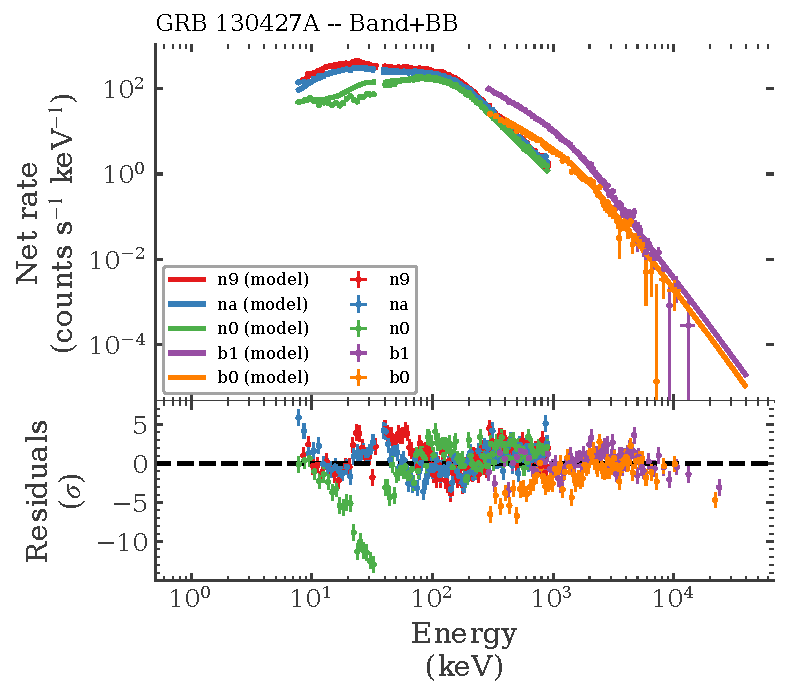
\includegraphics[width=0.46\textwidth]{two_break_figures/fig_spec_a.pdf}\hfill
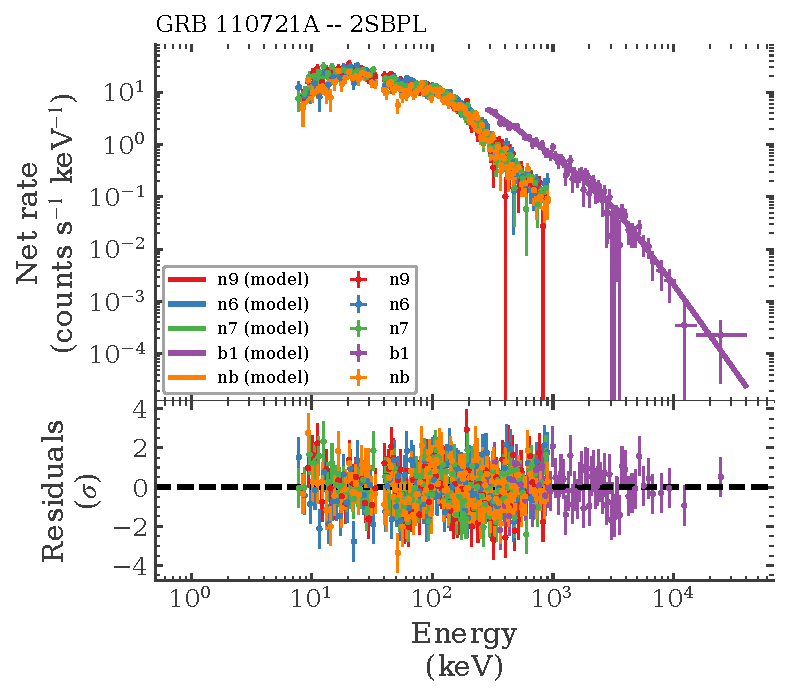
\includegraphics[width=0.46\textwidth]{two_break_figures/fig_spec_b.pdf}
\caption{Count spectra and residuals for the two emblematic curvature cases.
Left: a decisively blackbody-requiring bin of GRB~130427A ($8.7$--$11.0$~s)
fit with Band$+$BB, chosen away from the flux peak where pile-up may affect
this exceptionally bright burst \citep[cf.][]{Mei2025}; the narrow low-energy
residual structure in one NaI is of the kind attributed to response
calibration and intra-bin spectral evolution in very bright bursts
\citep[cf.][]{Ronchi2020}. Right: the most decisive two-break bin of
GRB~110721A ($0.5$--$2.0$~s) fit with the 2SBPL, with flat residuals across
8~keV--100~MeV (NaI, BGO, and LLE). Each color is one detector; solid lines
show the folded model.}
\label{fig:spec}
\end{figure*}

\begin{deluxetable}{lcc}
\tablecaption{Classification of the bins requiring curvature beyond a single
spectral break.\label{tab:curvsplit}}
\tablehead{\colhead{} & \colhead{$\daic>6$} & \colhead{$\daic\ge10$}}
\startdata
Curvature-required bins        & 166        & 108        \\
~~thermal-or-degenerate        & 151 (91\%) & 94 (87\%)  \\
~~two-break (2SBPL, decisive)  & 15 (9\%)   & 14 (13\%)  \\
\enddata
\tablecomments{Curvature is required when the best valid curved model
($+$BB or 2SBPL) improves on the best valid single-break model by the stated
\daic; ``decisive'' two-break additionally requires $\daic\ge10$ for the 2SBPL
over the SBPL. Two-break fractions are lower limits (Section~\ref{sec:fit}).}
\end{deluxetable}

\begin{figure*}[t]
\centering
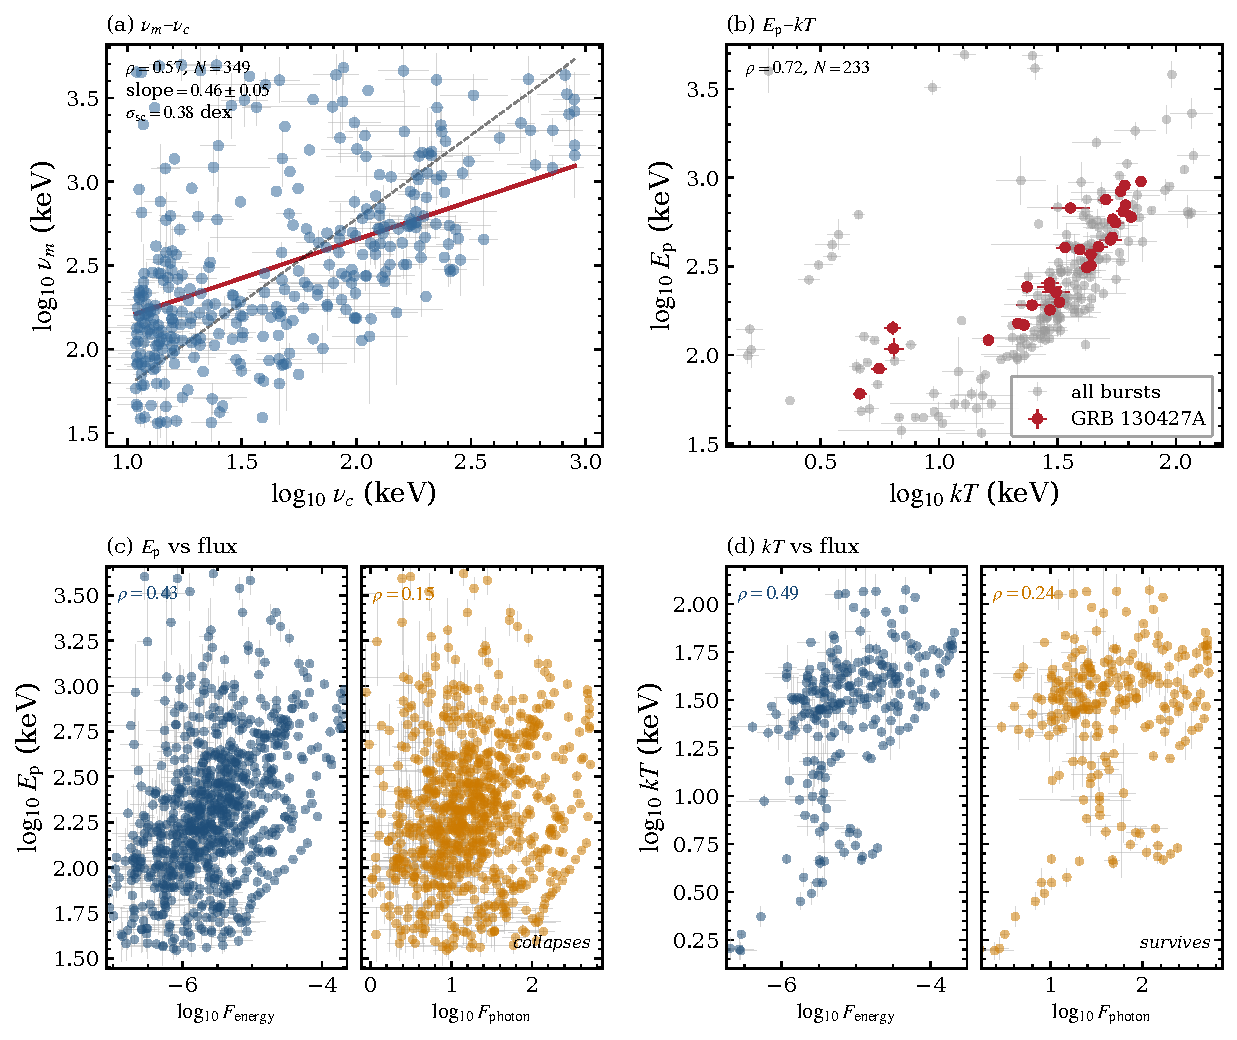
\includegraphics[width=0.92\textwidth]{two_break_figures/fig_corr.pdf}
\caption{Spectral-break and temperature correlations. (a) The two 2SBPL break
energies $\num$ vs $\nuc$ ($N=349$; red: \citealt{DAgostini2005}
errors-in-both-variables fit, slope $0.46\pm0.05$; dashed: 1:1). (b) The
$\Ep$--$\kT$ relation over the decisive-blackbody bins, with GRB~130427A
highlighted. (c) $\Ep$ vs energy flux (left, blue) and photon flux (right,
orange), sharing the $y$-axis: the correlation \emph{collapses} from
$\rho=0.43$ to $0.15$, showing it is largely induced by energy weighting.
(d) The same comparison for $\kT$: the correlation \emph{survives} in photon
flux ($\rho=0.24$; energy flux $0.49$), indicating a real thermal--intensity
link. Error bars are drawn where the fitted parameter is constrained
(relative uncertainty below 100\%; flux interval below 0.5~dex).}
\label{fig:corr}
\end{figure*}

% ============================================================================
